\section{Introduction}
\noindent Video inpainting aims to recover the missing contents of given videos, which can assist lots of practical applications, e.g., video restoration and augmented reality. Compared with image inpainting, video inpainting is much more challenging due to extra time dimension. It requires not only reasonable spatial structures but also stable temporal consistency. Specifically, directly applying 2D image inpainting algorithm \cite{yu2018free,Xiong_2019_CVPR} to individual frames is a sub-optimal choice, due to serious artificial effect, flickers and jitters. 

To exploit complementary neighboring information across frames, traditional patch-based methods \cite{patwardhan2007video,wexler2004space,newson2014video} recurrently copy the similar patches from unmasked regions and past them to the missing regions. 
\begin{figure}[t]
	\centering
	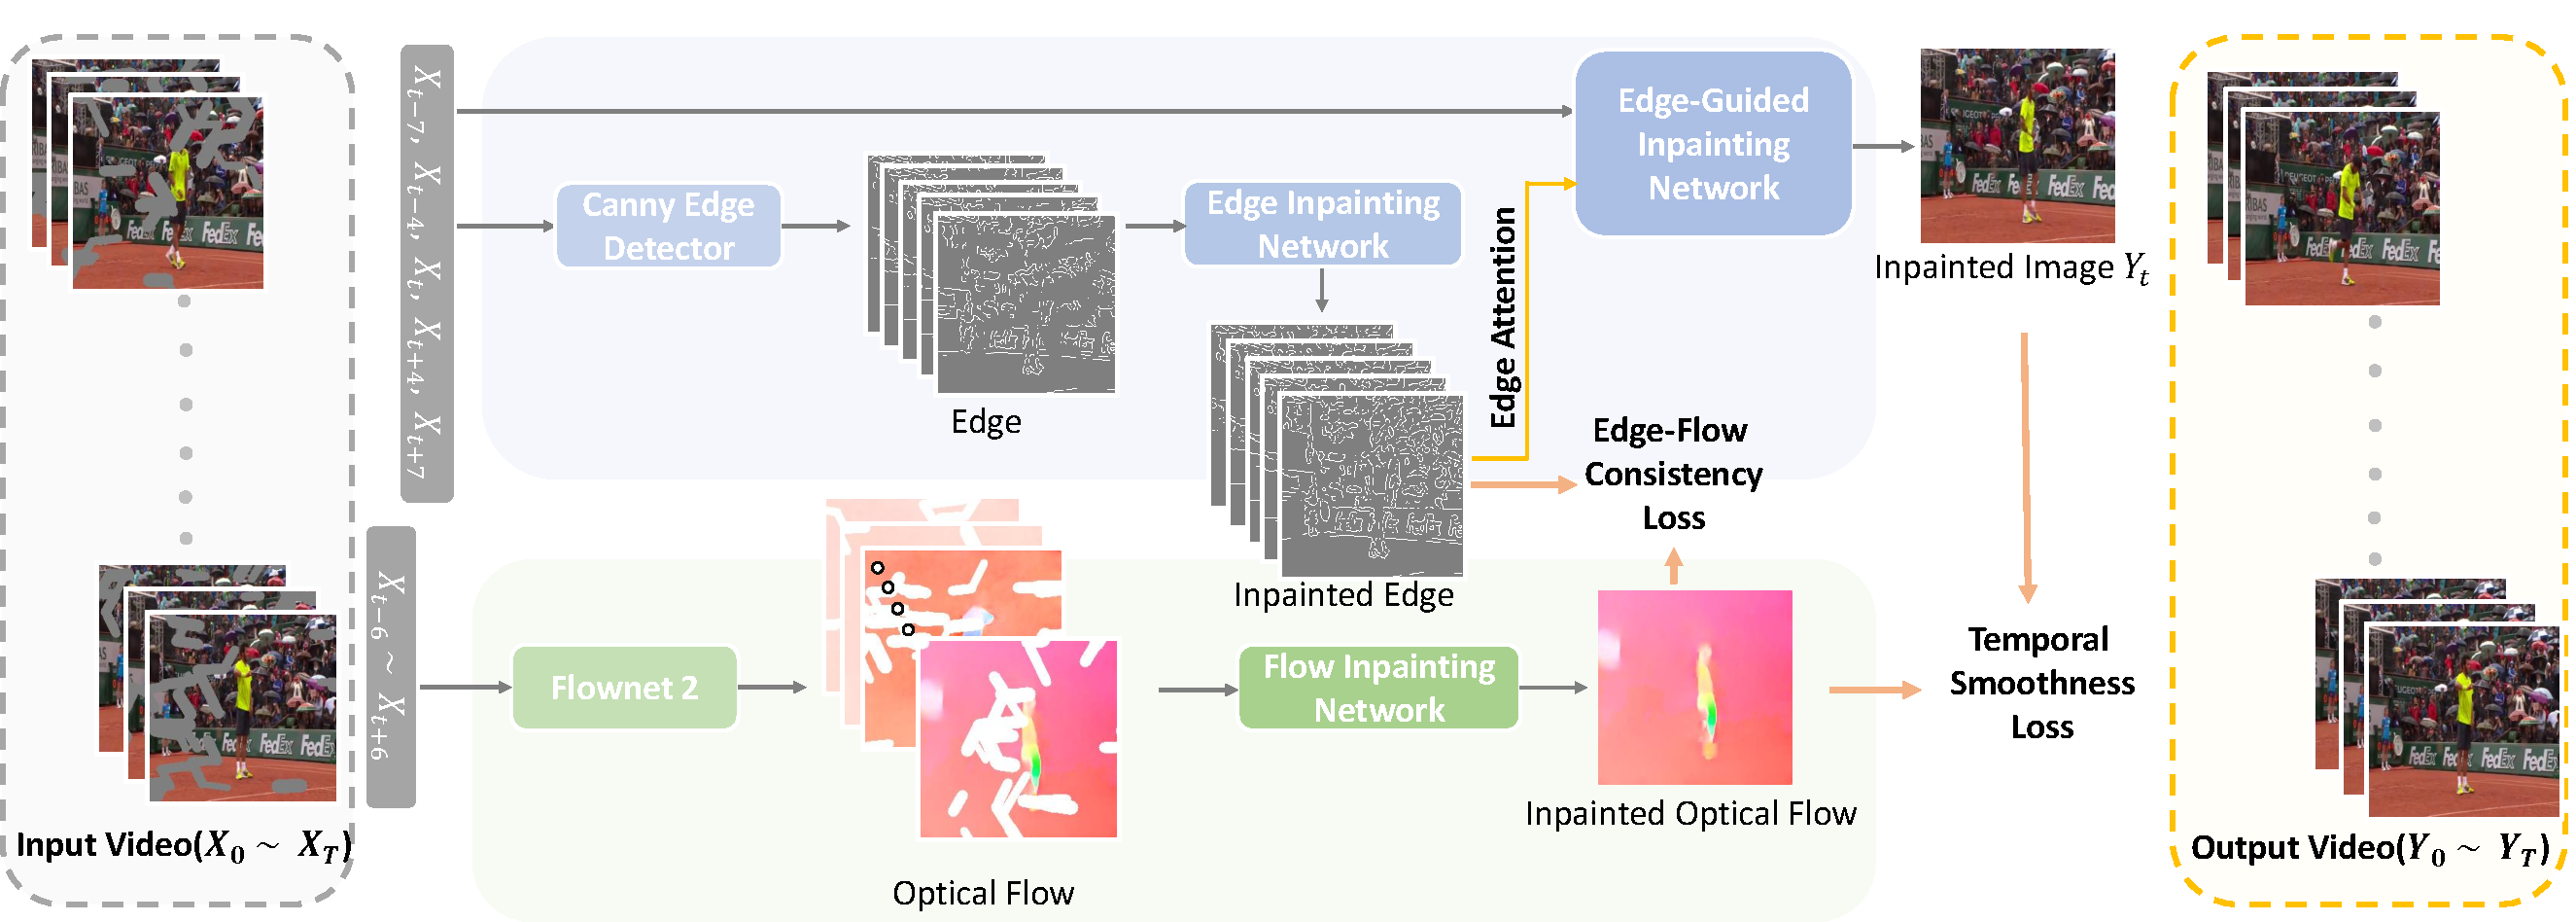
\includegraphics[width=1.0\columnwidth]{zong} % Reduce the figure size so that it is slightly narrower than the column. Don't use precise values for figure width.This setup will avoid overfull boxes. 
	\caption{The overall pipeline of SOVI. The ENet first completes the missing edge across frames. Then, under the guidance of structural edge, STINet can produce structure-preserved inpainting frame. Moreover, the FNet is designed to predict missing optical flow, which provides temporally consistency to the final result.}
	\label{zong}
\end{figure}
This kind of methods depends on a strong hypothesis that the missing content have precisely appeared in neighboring frames, which limits their generalization.
Recently, deep-learning based methods achieve state-of-the-art performance by treating a video as volume.
They utilize the CNNs, e.g., 3D convolution operation \cite{wang2019video}, to predict missing content with smooth motion, which is learned from training data.
Among these methods, optical flow is commonly used to temporally smooth the inpainted contents \cite{Xu_2019_CVPR,Kim_2019_CVPR,Kim_2019_CVPR1} by aggregating the contextual information from neighboring frames.
However, the auxiliary motion compensation brought by optical flow lacks detailed structural clues,~\emph{e.g.}~the inner textures of objects are usually missed in flow field, leading to deficient structure rationality.
Thus, how to obtain fine-detailed inpainting video remains an open problem.






In this paper, we present a novel structure-oriented video inpainting network (SOVI) that can collect and refine the structure information to improve the inpainting results. As shown in Fig.~\ref{zong}, our method consists of three modules, which are respectively the edge inpainting network (ENet), flow inpainting network (FNet), and spatio-temporal inpainting network (STINet).
Given frames with missing pixels, ENet first completes the edge maps that indicate the detailed structure information. Then, under the guidance of completed edge, STINet is developed to fill the missing colors and textures in a coarse-to-fine manner.
Specifically, a structure attention module is designed to capture the latent spatial relevance between video contents and structure edges.
Compared with original edge maps, the structure-texture relevance is easier to be embedded into STINet, which benefits fine-detailed frames generation.
Besides, the developed FNet can predict the missing optical flow, which provides auxiliary motion knowledge. Explicitly, a flow-edge consistency constraint and a temporal ensemble module are utilized to smoothen the edge maps and final inpainted frames, based on the motion tendency. Consequently, the inpainted frames by SOVI are not only detail-preserved but also temporal consistent.
%by simultaneously exploring optical flow and , to eliminate temporal flickers and enhance spatial detail. 
%  and FNet  and optical flow,  knowledge and motion tendency.
%according to learned structure knowledge and motion tendency from the training data,
%Instead of separate training, these two modules are
%This results in both edge-enhanced optical flow and temporally smooth edge. 
%Specifically, a structure enhancement mechanism is developed to extract and refine the structural clues in the completed edge and encode them into the STI.
% the optical flow is used by propagating complementary pixels from neighboring frames to current frame to alleviate artificial flickers and jitters.
Experiments on YouTubeVOS and DAVIS datasets show that the proposed method obtains new state-of-the-art performance with low time consumption, which demonstrates its superiority.

Our contributions can be summarized as follows.
\begin{itemize}
	\item A novel structure-oriented video inpainting method is proposed, which can generate structural reasonable and temporal coherent inpainted frames.
	
	\item We introduce an edge inpainting network to predict the missing edges. Besides, a novel structure attention module is designed to capture the spatial relevance between video contents and structure edges, which is easily to be embedded into video inpainting network. %With edge collection and structure embedding, we demonstrate the significance of detailed structure in video inpainting. 
	%to structure information is well represented and encoded in video inpainting via . 
	\item A flow-guided warping and temporal ensemble module are developed to enhance temporal consistency for video inpainting, with a flow inpainting network.
	%	Optical flow is used to enhance temporal consistency, which 

	
	%	We propose a novel structure- for video inpainting, by simultaneously exploring optical flow and structural clues to eliminate temporal flickers and enhance structure detail. 
	%	 A flow-edge consistency loss is developed to associate the optical flow and structure edges, which can boost each other.
	%	\item  a structure enhancement mechanism is  designed, which can promote the video inpainting.	
	
\end{itemize}





\section{Related Work}
\subsubsection{Traditional Image/Video Inpainting }
Traditional image/video methods can be divided into two kinds, diffusion-based and patch-based methods. The Diffusion-based method \cite{bertalmio2000image,ballester2001filling} gradually propagates contents from boundaries to the missing holes. However, this kind of method fails to handle large holes. 
The patch-based method \cite{bertalmio2003simultaneous,efros2001image} formulates the task as a patch-based optimization problem, which is mostly used. It fills the missing image contents by borrowing and aggregating the most similar patches from known regions. \cite{patwardhan2007video} further extends the task to video inpainting by searching patches in across frames. \cite{newson2014video} enhances the quality of video inpainting by using a video version of PatchMatch algorithm. Then, \cite{huang2016temporally} proposes completing the missing optical flow to alleviate the temporal artifacts and enforce temporal consistency. 
However, traditional methods assume that there should exist complementary contents in known regions, which can not synthesize unseen appearances. Besides, propagation process makes these methods suffer from high computational complexity, which causes the limitation of practical usage. 

\subsubsection{CNN-based Image/Video Inpainting }
Recently, deep learning methods can capture high-level semantic information of images/videos, which have achieved tremendous progress. \cite{xie2012image} first introduces convolution neural network (CNN) to synthesize small unknown regions and denoise in images. To make the generated results more realistic, \cite{pathak2016context} uses generative adversarial network to jointly train a generator and a discriminator. Then, \cite{iizuka2017globally} proposes using two discriminators to constrain both global and local coherence of image contents. However, methods aforementioned usually handle the square masks, which produce artificial when recovering challenging holes of irregular shapes. To solve this,
 \cite{liu2018partialinpainting} designs a network which utilizes the partial convolution. Later, \cite{yu2018free} introduces gated convolution to learn a dynamic feature selection mechanism in CNN.  \cite{nazeri2019edgeconnect} introduces an edge generator to refine generated structure in image inpainting. These image inpainting methods can obtain plausible synthesized images. However, directly extending these state-of-the-art image inpainting methods to video domain is not an optimal solution, which will generate videos with serious temporal flickers, artifacts and jitters. Besides, Image inpainting methods can not utilize useful complementary information in neighboring frames. To obtain spatio-temporal consistent inpainted video, some methods have been proposed recently.
\cite{wang2019video} proposes CombCN to capture both temporal and spatial consistency, which is the first to use CNN-based method in video inpainting. \cite{Xu_2019_CVPR} proposes a stacked convolution network to predict missing motion field and regards video inpainting as a pixel propagation problem. \cite{Kim_2019_CVPR} automatically removes texts in videos without mask indications, which aggregates temporal features from encoder to decoder and applies a recurrent feedback. \cite{Kim_2019_CVPR1} introduces convolutional LSTM and temporal feature aggregation to obtain temporal consistency and learn information from neighboring frames. However, these existing methods neglect the importance of structure information in video inpainting, which will cause the blurry details and structural cracks in generated videos. 

To tackle these issues, we propose a novel structure-oriented video inpainting network (SOVI) based on CNN.
 Different from the methods above, SOVI
takes the effect of structure information into consideration. In our network, we collect and refine the structure information to enhance the final generated video. Specifically, a structure attention module is introduced to learn latent correlation between video contents and structure. Besides, temporal consistency is also guaranteed through flow-guided warping and temporal ensemble module. Finally, we can generate spatio-temporal consistent inpainted video. 